\documentclass{article}
\usepackage{tikz}
\usepackage{xcolor}
\usetikzlibrary{patterns}
\usetikzlibrary{shapes,arrows}
\usepackage{pgfplots}

\begin{document}
\center
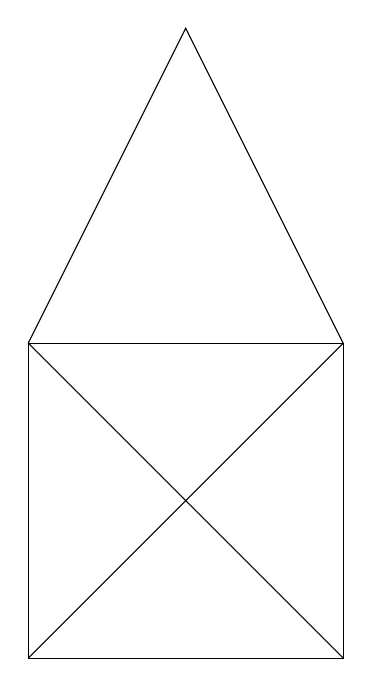
\begin{tikzpicture}[scale=2.0]
	\draw (0,2) -- (1,4) -- (2,2);
    \draw (0,0) -- (2,0) -- (2,2) -- (0,2) -- cycle;
    \draw (0,0) -- (2,2);
    \draw (0,2) -- (2,0);    
\end{tikzpicture}
\center
\bigbreak\bigbreak\bigbreak\bigbreak\bigbreak
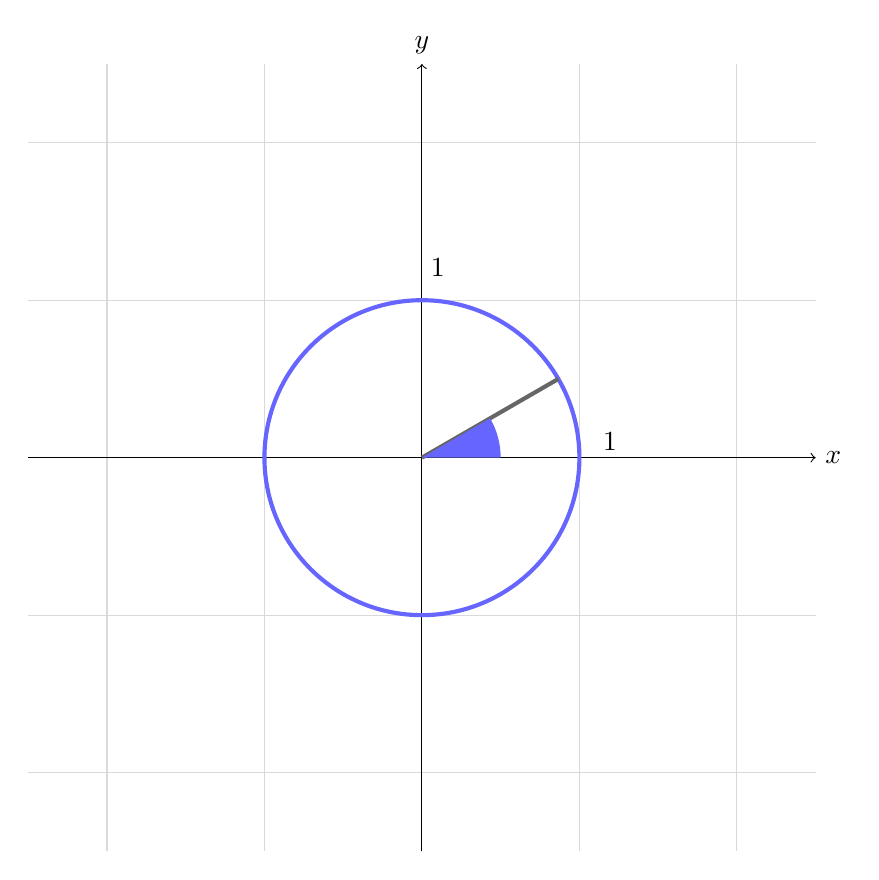
\begin{tikzpicture}[scale=2.0]
	\draw[gray!30] (-2.5,-2.5) grid (2.5,2.5);
    \draw[->] (-2.5,0) -- (2.5,0) node[right] {$x$};
    \draw[->] (0,-2.5) -- (0,2.5) node[above] {$y$};
    \foreach \x in {1}
        \draw (\x,-0.1) -- (\x,0.1) node[right=5pt] {$\x$};
         \foreach \y in {1}
        \draw (-0.1,\y) -- (0.1,\y) node[above=5pt] {$\y$};
	\draw[blue!60, line width=1.5pt] (0,0) circle (1);
 	\draw[black!60, line width=1.5pt] (0,0) -- (30:1);
  	\fill[blue!60] (0,0) -- (0:0.5) arc (0:30:0.5) -- cycle;
\end{tikzpicture}
\bigbreak\bigbreak\bigbreak\bigbreak\bigbreak
\center
\begin{tikzpicture}
    % Téglalap csúcsainak koordinátái
    \coordinate (A) at (0,0);
    \coordinate (B) at (3,0);
    \coordinate (C) at (3,2);
    \coordinate (D) at (0,2);

    % Téglalap rajzolása
    \draw (A) -- (B) -- (C) -- (D) -- cycle;
    ;
\end{tikzpicture}

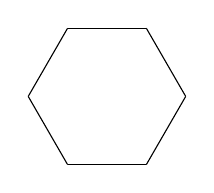
\begin{tikzpicture}[scale=0.5]

   \foreach \x in {0,60,...,300}
        \draw (\x:2) -- ({\x+60}:2);
\end{tikzpicture}

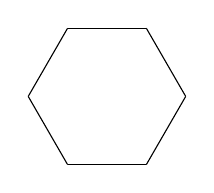
\begin{tikzpicture}[scale=0.5]

   \foreach \x in {0,60,...,300}
        \draw (\x:2) -- ({\x+60}:2);
\end{tikzpicture}

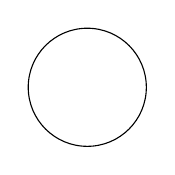
\begin{tikzpicture}
    % Körcikk rajzolása
    \draw (2, 0.75) circle (0.75);
\end{tikzpicture}

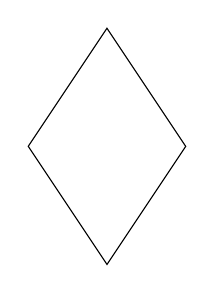
\begin{tikzpicture}
    % Romnusz csúcsainak koordinátái
    \coordinate (A) at (2,0);
    \coordinate (B) at (3,1.5);
    \coordinate (C) at (2,3);
    \coordinate (D) at (1,1.5);

    % Rombusz rajzolása
    \draw (A) -- (B) -- (C) -- (D) -- cycle;
\end{tikzpicture}

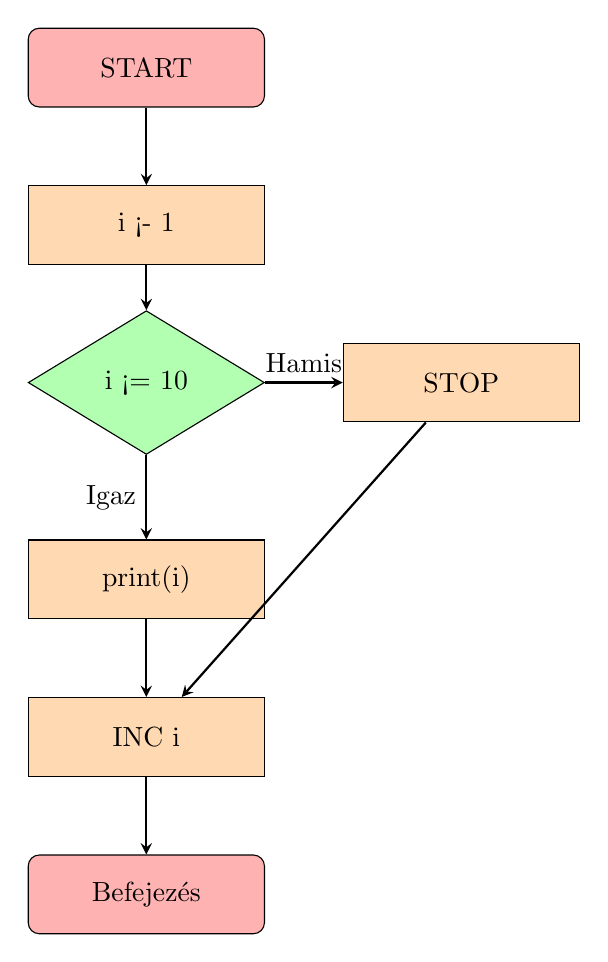
\begin{tikzpicture}[node distance=2cm, auto]

% Folyamatábra alakzatok definiálása
\tikzstyle{startstop} = [rectangle, rounded corners, minimum width=3cm, minimum height=1cm, text centered, draw=black, fill=red!30]
\tikzstyle{process} = [rectangle, minimum width=3cm, minimum height=1cm, text centered, draw=black, fill=orange!30]
\tikzstyle{decision} = [diamond, minimum width=3cm, minimum height=1cm, text centered, draw=black, fill=green!30]
\tikzstyle{arrow} = [thick,->,>=stealth]

% Folyamatábra elemek
\node (start) [startstop] {START};
\node (input) [process, below of=start] {i <- 1};
\node (decision) [decision, below of=input] {i <= 10};
\node (process1) [process, below of=decision, yshift=-0.5cm] {print(i)};
\node (process2) [process, right of=decision, xshift=2cm] {STOP};
\node (output) [process, below of=process1] {INC i};
\node (stop) [startstop, below of=output] {Befejezés};

% Folyamatábra vonalak
\draw [arrow] (start) -- (input);
\draw [arrow] (input) -- (decision);
\draw [arrow] (decision) -- node[anchor=east] {Igaz} (process1);
\draw [arrow] (decision) -- node[anchor=south] {Hamis} (process2);
\draw [arrow] (process2) -- (output);
\draw [arrow] (process1) -- (output);
\draw [arrow] (output) -- (stop);
\end{tikzpicture}


\begin{tikzpicture}
\begin{axis}[
    xlabel=$x$,
    ylabel={$y$},
    domain=0:2*pi,
    samples=100,
    axis lines=middle,
    legend pos=outer north east,
]

\addplot[red,thick]{sin(deg(x))};
\addplot[blue,thick]{cos(deg(x))};
\legend{$\sin(x)$, $\cos(x)$}
\mark=x
\end{axis}
\end{tikzpicture}

\end{document}
